\documentclass[tikz,border=8pt]{standalone}
\usepackage[T1]{fontenc}
\usepackage{helvet}
\renewcommand{\familydefault}{\sfdefault}
\usetikzlibrary{arrows.meta}

\definecolor{queryfill}{HTML}{DFF7F3}
\definecolor{queryborder}{HTML}{1BA99C}
\definecolor{corpusfill}{HTML}{FFF4D6}
\definecolor{corpusborder}{HTML}{D9A441}
\definecolor{bm25fill}{HTML}{FFE9C8}
\definecolor{bm25border}{HTML}{D88922}
\definecolor{llmfill}{HTML}{E9EDFF}
\definecolor{llmborder}{HTML}{6979C9}
\definecolor{nodefill}{HTML}{E8F2FF}
\definecolor{nodeborder}{HTML}{4E8CD8}
\definecolor{outfill}{HTML}{E7F6E7}
\definecolor{outborder}{HTML}{4FA64F}
\definecolor{softgray}{HTML}{F4F7FB}
\definecolor{darkline}{HTML}{333333}

\tikzset{
  card/.style={rectangle, rounded corners=5pt, align=center, draw=darkline, line width=0.8pt, minimum height=0.82cm, font=\small},
  query/.style={card, fill=queryfill, draw=queryborder, minimum width=2.05cm},
  corpus/.style={card, fill=corpusfill, draw=corpusborder, minimum width=2.25cm},
  bm25/.style={card, fill=bm25fill, draw=bm25border, minimum width=2.55cm, font=\small\bfseries},
  llm/.style={card, fill=llmfill, draw=llmborder, minimum width=2.6cm, font=\small\bfseries},
  artifact/.style={card, fill=white, minimum width=2.75cm},
  output/.style={card, fill=outfill, draw=outborder, minimum width=2.75cm},
  softbox/.style={rectangle, rounded corners=8pt, draw=darkline, fill=softgray, line width=0.7pt},
  doc/.style={rectangle, rounded corners=4pt, fill=corpusfill, draw=corpusborder, line width=0.7pt, minimum width=0.42cm, minimum height=0.58cm},
  node/.style={circle, fill=nodefill, draw=nodeborder, line width=0.7pt, minimum size=0.29cm},
  finalnode/.style={circle, fill=outfill, draw=outborder, line width=0.7pt, minimum size=0.29cm},
  phase/.style={font=\small\bfseries, align=center},
  flow/.style={-{Latex[length=2.2mm]}, line width=0.85pt, draw=darkline},
  faint/.style={dashed, darkline, opacity=0.32}
}

\begin{document}
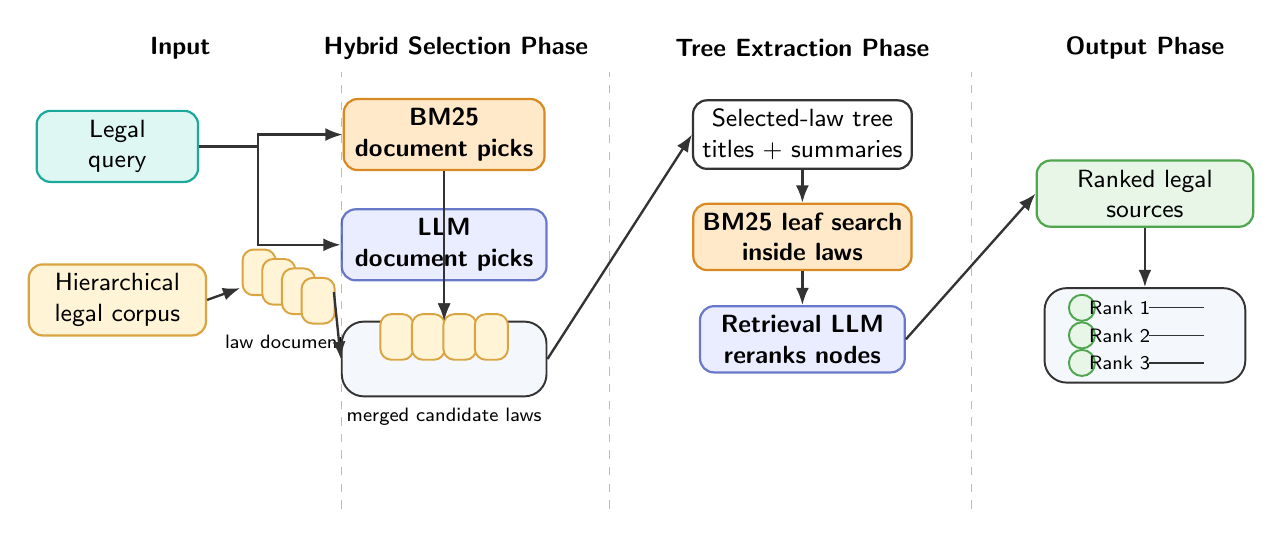
\begin{tikzpicture}

\node[phase] at (1.1,5.85) {Input};
\node[phase] at (4.6,5.85) {Hybrid Selection Phase};
\node[phase] at (9.0,5.85) {Tree Extraction Phase};
\node[phase] at (13.35,5.85) {Output Phase};

\node[query] (query) at (0.3,4.6) {Legal\\query};
\node[corpus] (corpus) at (0.3,2.65) {Hierarchical\\legal corpus};

\foreach \x/\y in {2.1/3.0,2.35/2.88,2.6/2.76,2.85/2.64} {
  \node[doc] at (\x,\y) {};
}
\node[font=\scriptsize] at (2.48,2.12) {law documents};

\node[bm25] (bm25doc) at (4.45,4.75) {BM25\\document picks};
\node[llm] (llmdoc) at (4.45,3.35) {LLM\\document picks};
\node[softbox, minimum width=2.6cm, minimum height=0.95cm] (merged) at (4.45,1.9) {};
\foreach \x in {3.85,4.25,4.65,5.05} {
  \node[doc] at (\x,2.18) {};
}
\node[font=\scriptsize] at (4.45,1.17) {merged candidate laws};

\node[artifact] (treeview) at (9.0,4.75) {Selected-law tree\\titles + summaries};
\node[bm25] (leafbm25) at (9.0,3.45) {BM25 leaf search\\inside laws};
\node[llm] (rerank) at (9.0,2.15) {Retrieval LLM\\reranks nodes};

\node[output] (sources) at (13.35,4.0) {Ranked legal\\sources};
\node[softbox, minimum width=2.55cm, minimum height=1.2cm] (rankbox) at (13.35,2.2) {};
\foreach \y/\lab in {2.55/1,2.2/2,1.85/3} {
  \node[finalnode] at (12.55,\y) {};
  \node[font=\scriptsize] at (13.03,\y) {Rank \lab};
  \draw[darkline, line width=0.5pt] (13.4,\y) -- (14.1,\y);
}

\draw[flow] (query.east) -- ++(0.75,0) |- (bm25doc.west);
\draw[flow] (query.east) -- ++(0.75,0) |- (llmdoc.west);
\draw[flow] (corpus.east) -- (1.86,2.8);
\draw[flow] (3.05,2.75) -- (merged.west);
\draw[flow] (bm25doc) -- (merged);
\draw[flow] (llmdoc) -- (merged);
\draw[flow] (merged.east) -- (treeview.west);
\draw[flow] (treeview) -- (leafbm25);
\draw[flow] (leafbm25) -- (rerank);
\draw[flow] (rerank.east) -- (sources.west);
\draw[flow] (sources) -- (rankbox);

\draw[faint] (3.15,0.0) -- (3.15,5.55);
\draw[faint] (6.55,0.0) -- (6.55,5.55);
\draw[faint] (11.15,0.0) -- (11.15,5.55);

\end{tikzpicture}
\end{document}
